
\chapter*{Dev Notes}

\section{Concretizing less does not infer spuriousness}

\subsection{Concrete AF}

\begin{center}
	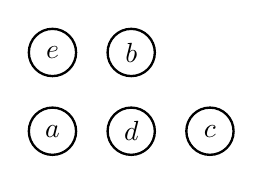
\begin{tikzpicture}
		\def \ax{0.0} \def \ay{-1.0}
		\def \bx{1.0} \def \by{0.0}
		\def \cx{2.0} \def \cy{-1.0}
		\def \dx{1.0} \def \dy{-1.0}
		\def \ex{0.0} \def \ey{0.0}
  
        % Singletons
        \draw[line width=0.3mm] (\ax,\ay)  circle (0.3) node[anchor=center]{$a$};
        \draw[line width=0.3mm] (\bx,\by)  circle (0.3) node[anchor=center]{$b$};
        \draw[line width=0.3mm] (\cx,\cy)  circle (0.3) node[anchor=center]{$c$};
        \draw[line width=0.3mm] (\dx,\dy)  circle (0.3) node[anchor=center]{$d$};
        \draw[line width=0.3mm] (\ex,\ey)  circle (0.3) node[anchor=center]{$e$};
		% Attacks
		\DrawAttackHorizontal{R}{\ex}{\ey}{\bx}{\by}
		\DrawAttackHorizontal{L}{\dx}{\dy}{\ax}{\ay}
		\DrawAttackHorizontal{R}{\dx}{\dy}{\cx}{\cy}

		\DrawAttackVertical{B}{\bx}{\by}{\dx}{\dy}
		\DrawSelfAttackRightSingleton{\bx}{\by}
		\DrawSelfAttackRightSingleton{\cx}{\cy}
        
	\end{tikzpicture}
\end{center}
\textbf{Stable Sets:} $\{ d, e\}$

\subsection{Abstract AF}
\begin{center}
	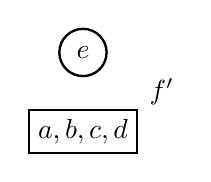
\begin{tikzpicture}
		\def \ex{0.0} \def \ey{ 0.0}
		\def \fx{0.0} \def \fy{-1.0}
        % Clusters
        \node[rectangle, draw, line width=0.3mm] at (\fx, \fy) {$a,b,c,d$};
		\node at (1, -0.5) {$f'$};
        % Singletons
        \draw[line width=0.3mm] (\ex,\ey)  circle (0.3) node[anchor=center]{$e$};
		% Attacks
		\DrawAttackVertical{U}{\fx}{\fy}{\ex}{\ey}
		\DrawSelfAttackLeftTopCluster{\fx-0.63}{\fy + 0.3}
	\end{tikzpicture}
\end{center}
\textbf{Stable Sets:} $\{ f', e\}$, $\{ e\}$

Abstract AF is \textbf{spurious} to concrete AF because set $\{ e\}$.



\subsection{Concretized AF (b,d) Grounded}
\begin{center}
	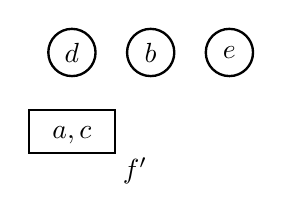
\begin{tikzpicture}
		\def \bx{1.0} \def \by{0.0}
		\def \dx{0.0} \def \dy{0.0}
		\def \ex{2.0} \def \ey{0}
		\def \fx{0.0} \def \fy{-1.0}
        % Clusters
        \node[rectangle, draw, line width=0.3mm] at (\fx, \fy) {$\phantom{d}a, c\phantom{d}$};
		\node at (0.8, -1.5) {$f'$};
        % Singletons
        \draw[line width=0.3mm] (\bx,\by)  circle (0.3) node[anchor=center]{$b$};
        \draw[line width=0.3mm] (\dx,\dy)  circle (0.3) node[anchor=center]{$d$};
        \draw[line width=0.3mm] (\ex,\ey)  circle (0.3) node[anchor=center]{$e$};
		% Attacks
		\DrawAttackHorizontal{B}{\bx}{\by}{\dx}{\dy}
		\DrawAttackHorizontal{R}{\bx}{\by}{\ex}{\ey}

		\DrawAttackVertical{D}{\dx}{\dy}{\fx}{\fy}

		\DrawSelfAttackRightSingleton{\bx}{\by}

		\DrawSelfAttackLeftTopCluster{\fx-0.45}{\fy + 0.3}
        
	\end{tikzpicture}
\end{center}
\textbf{Stable Sets:} $\{ d, e\}$, $\{ d, e, f'\}$

Concretized AF (b, d) is \textbf{spurious} to concrete AF because set $\{ d, e, f'\}$.


\subsection{Concretized AF (b)}
\begin{center}
	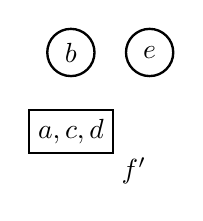
\begin{tikzpicture}
		\def \bx{0.0} \def \by{ 0.0}
		\def \ex{1.0} \def \ey{ 0.0}
		\def \fx{0.0} \def \fy{-1.0}
        % Clusters
        \node[rectangle, draw, line width=0.3mm] at (\fx, \fy) {$a,c,d$};
		\node at (0.8, -1.5) {$f'$};
        % Singletons
        \draw[line width=0.3mm] (\bx,\by)  circle (0.3) node[anchor=center]{$b$};
        \draw[line width=0.3mm] (\ex,\ey)  circle (0.3) node[anchor=center]{$e$};
		% Attacks
		\DrawAttackHorizontal{L}{\ex}{\ey}{\bx}{\by}
		\DrawAttackVertical{B}{\bx}{\by}{\fx}{\fy}

		\DrawSelfAttackRightSingleton{\bx}{\by}

		\DrawSelfAttackLeftTopCluster{\fx-0.45}{\fy + 0.3}
	\end{tikzpicture}
\end{center}
\textbf{Stable Sets:} $\{ f', e\}$

Concretized AF (e) is \textbf{faithful} to concrete AF.


